\documentclass[a4paper,11pt]{article}
\usepackage{ctex}
\usepackage{enumerate}
\usepackage{times}
\usepackage{mathptmx}
\usepackage{amsmath}
\usepackage{amssymb}
\usepackage{tikz}
\usepackage{clrscode3e}
\usepackage{url}
\usepackage[top=2cm, bottom=2cm, left=2cm, right=2cm]{geometry}

\allowdisplaybreaks[4]
\renewcommand{\labelenumi}{\textbf{\emph{\alph{enumi}}.}}
\newcommand{\NIL}{\const{nil}}
\newcommand{\od}{\mathop{\mathrm{od}}}
\begin{document}
  \title{����~2-16~��ҵ}
  \author{��������ۿԴ \and ѧ�ţ�161240004}
  \date{}
  \maketitle

  \section{[TC] Problem 22.1-3}
  For adjacency-list representation:
  \begin{codebox}
  \Procname{$\proc{Transpose}(G)$}
  \li let $\id{Adj}[1 \twodots |V(G)|]$ be a new array of lists
  \li \For $i \gets 1$ \To $|V(G)|$
  \li \Do  \For each $e$ in $\attrib{G}{Adj}[i]$
  \li      \Do $\attribii{Adj[e]}{insert}(i)$
           \End
      \End
  \li \Return graph $(V(G), \id{Adj})$
  \end{codebox} \par
  For adjacency-matrix representation:
  \begin{codebox}
  \Procname{$\proc{Transpose}(G)$}
  \li let $\id{A}[1 \twodots |V(G)|, 1 \twodots |V(G)|]$ be a new array
  \li \For $i \gets 1$ \To $|V(G)|$
  \li \Do  \For $j \gets 1$ \To $|V(G)|$
  \li      \Do $A(i, j) \gets \attrib{G}{A}(j, i)$
           \End
      \End
  \li \Return graph $(V(G), A)$
  \end{codebox}

  \section{[TC] Problem 22.1-8}
  If we use hash table with collision resolution by chaining, the expected time to determine whether an edge is in the graph is $O(1 + \alpha)$, where $\alpha$ is the load factor. (We will not adopt open addressing, because it is no better than adjacency-matrix, i.e. direct-address tables) \par
  The disadvantage of this scheme is that, we still need a great number of memory space, even if the graph is very sparse. \par
  Instead of a hash table, we can use binary search tree as array entry $\id{Adj[u]}$, containing the vertices $v$ for which $(u, v) \in E$. This alternative requires $O(\log \od(u))$ time for determining whether an edge is in the graph, where $\od(u)$ is the out-degree of $u$, usually worse than hash table.

  \section{[TC] Problem 22.2-3}
  In \proc{BFS}, whether a vertex is black or gray does not affect the order in which the statements are executed, so we can remove line 18\footnote{According to the errata sheet (\url{http://www.cs.dartmouth.edu/~thc/clrs-bugs/bugs-3e.php}), the problem should be ``... if line 18 was removed''. This error has been corrected in the third printing of this book.}, i.e. leave the vertex gray after all its white adjacent nodes have been inserted to the queue, without changing the result the procedure produces.

  \section{[TC] Problem 22.2-4}
  Instead of going through the adjacency list, we have to go through a row of the adjacency matrix to determine the edges in the graph, which takes a running time of $O(|V|^2)$.

  \section{[TC] Problem 22.2-5}
  By Theorem 22.5, after BFS is done, $\attrib{u}{d}$ is the distance from the source to $u$. Changing the order of the vertices in each adjacency list does not change the graph the lists represents, thus does not change $\attrib{u}{d}$. \par
  For the graph shown in Figure 22.3, if the adjacency lists are: \par
  \vspace{0.2cm}
  \begin{centering}
  \begin{tabular}{c|c|c|c|c|c|c|c|c}
      \hline
      vertex & $r$ & $s$ & $t$ & $u$ & $v$ & $w$ & $x$ & $y$ \\ \hline
      \id{Adj} & $v, s$ & $r, w$ & $w, x, u$ & $t, x, y$ & $r$ & $s, t, x$ & $w, t, u, y$ & $x, u$ \\ \hline
  \end{tabular}\par
  \end{centering}
  \vspace{0.2cm}
  the breadth-first tree computed by BFS (from $s$) is: \par
  \begin{centering}
    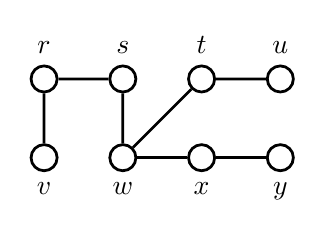
\begin{tikzpicture}[line width = 1pt,
                      solid/.style = {circle, draw, fill = black, minimum size = 0.1cm},
                      empty/.style = {circle, draw, fill = white, minimum size = 0.1cm}]
    \node [empty, label=above:$r$] (r) at (1, 1){};
    \node [empty, label=above:$s$] (s) at (2, 1){};
    \node [empty, label=above:$t$] (t) at (3, 1){};
    \node [empty, label=above:$u$] (u) at (4, 1){};
    \node [empty, label=below:$v$] (v) at (1, 0){};
    \node [empty, label=below:$w$] (w) at (2, 0){};
    \node [empty, label=below:$x$] (x) at (3, 0){};
    \node [empty, label=below:$y$] (y) at (4, 0){};

    \draw (v) -- (r) -- (s) -- (w) -- (t) -- (u);
    \draw (w) -- (x) -- (y);
    \end{tikzpicture} \par
  \end{centering}
  If we change to the order of the vertices in the adjacency list of $x$: \par
  \vspace{0.2cm}
  \begin{centering}
    \begin{tabular}{c|c|c|c|c|c|c|c|c}
      \hline
      vertex & $r$ & $s$ & $t$ & $u$ & $v$ & $w$ & $x$ & $y$ \\ \hline
      \id{Adj} & $v, s$ & $r, w$ & $w, x, u$ & $t, x, y$ & $r$ & $s, x, t$ & $w, t, u, y$ & $x, u$ \\ \hline
    \end{tabular} \par
  \end{centering}
  \vspace{0.2cm}
  the breadth-first tree will be: \par
  \begin{centering}
    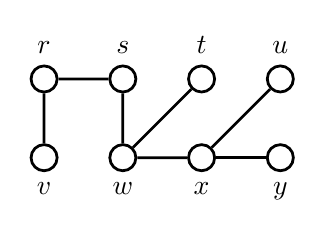
\begin{tikzpicture}[line width = 1pt,
                      solid/.style = {circle, draw, fill = black, minimum size = 0.1cm},
                      empty/.style = {circle, draw, fill = white, minimum size = 0.1cm}]
    \node [empty, label=above:$r$] (r) at (1, 1){};
    \node [empty, label=above:$s$] (s) at (2, 1){};
    \node [empty, label=above:$t$] (t) at (3, 1){};
    \node [empty, label=above:$u$] (u) at (4, 1){};
    \node [empty, label=below:$v$] (v) at (1, 0){};
    \node [empty, label=below:$w$] (w) at (2, 0){};
    \node [empty, label=below:$x$] (x) at (3, 0){};
    \node [empty, label=below:$y$] (y) at (4, 0){};

    \draw (v) -- (r) -- (s) -- (w) -- (t);
    \draw (w) -- (x) -- (u);
    \draw (x) -- (y);
    \end{tikzpicture} \par
  \end{centering}

  \section{[TC] Problem 22.3-6}
    For every edge $(u, v)$ ($\attrib{u}{d} < \attrib{v}{d}$), if $(u, v)$ is encountered first, then $v$ must remain unvisited, because $(v, u)$ will be encountered when visiting $v$. Hence $(u, v)$ is a tree edge. If $(v, u)$ is encountered first, then both $u, v$ are visited, and thus $(u, v)$ is a back edge. \par
    Since, in an undirected graph, every edge is either a tree edge or a black edge, we conclude that $(u, v)$ ($\attrib{u}{d} < \attrib{v}{d}$) is encountered first iff $(u, v)$ is a tree edge, and $(v, u)$ ($\attrib{u}{d} < \attrib{v}{d}$) is encountered first iff $(u, v)$ is a back edge. Therefore, these two schemes are equivalent.

  \section{[TC] Problem 22.3-7}
  \begin{codebox}
  \Procname{$\proc{DFS}(G)$}
  \li $time \gets 0$
  \li let $S$ be a new stack
  \li \For each vertex $u \in \attrib{G}{V}$
  \li \Do  $\attrib{u}{color} \gets \const{white}$
  \li      $\attrib{u}{\pi} \gets \NIL$
  \li      $\attrib{S}{push}(u)$
      \End
  \li \While $S$ is not empty
  \li \Do $u \gets \attrib{S}{pop}()$
  \li     \If $\attrib{u}{color} \isequal \const{white}$
  \li     \Do $time \gets time + 1$
  \li         $\attrib{u}{d} \gets time$
  \li         $\attrib{u}{color} \gets \const{gray}$
  \li         $\attrib{S}{push}(u)$
  \li         \For each vertex $v \in \attrib{G}{Adj}[u]$
  \li         \Do  \If $\attrib{v}{color} \isequal \const{white}$
  \li              \Do $\attrib{v}{\pi} \gets u$
  \li                  $\attrib{S}{push}(v)$
                   \End
              \End
  \li     \ElseIf $\attrib{u}{color} \isequal \const{gray}$
  \li     \Do $\attrib{u}{color} \gets \const{black}$
  \li         $time \gets time + 1$
  \li         $\attrib{u}{f} \gets time$
          \End
      \End
  \end{codebox}

  \section{[TC] Problem 22.3-8}
  Consider the following graph: \par
  \vspace{0.2cm}
  \begin{centering}
    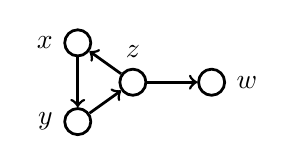
\begin{tikzpicture}[line width = 1pt,
                      solid/.style = {circle, draw, fill = black, minimum size = 0.1cm},
                      empty/.style = {circle, draw, fill = white, minimum size = 0.1cm}]
    \node [empty, label=left:$x$] (a) at (0, 0){};
    \node [empty, label=left:$y$] (b) at (0, -1){};
    \node [empty, label=above:$z$] (c) at (0.7, -0.5){};
    \node [empty, label=right:$w$] (d) at (1.7, -0.5){};
    \draw [->] (c) -- (a);
    \draw [->] (a) -- (b);
    \draw [->] (b) -- (c);
    \draw [->] (c) -- (d);
    \end{tikzpicture} \par
  \end{centering}
  In this graph, there exists a path from $y$ to $w$. If we perform depth-first search on this graph from $z$ in the order $z, x, y, w$, the depth-first forest is: \par
  \vspace{0.2cm}
  \begin{centering}
    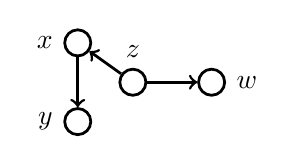
\begin{tikzpicture}[line width = 1pt,
                      solid/.style = {circle, draw, fill = black, minimum size = 0.1cm},
                      empty/.style = {circle, draw, fill = white, minimum size = 0.1cm}]
    \node [empty, label=left:$x$] (a) at (0, 0){};
    \node [empty, label=left:$y$] (b) at (0, -1){};
    \node [empty, label=above:$z$] (c) at (0.7, -0.5){};
    \node [empty, label=right:$w$] (d) at (1.7, -0.5){};
    \draw [->] (c) -- (a);
    \draw [->] (a) -- (b);
    \draw [->] (c) -- (d);
    \end{tikzpicture} \par
  \end{centering}
  In such order of DFS, $\attrib{y}{d} < \attrib{w}{d}$, however, $w$ is not a descendant of $y$ in this forest.

  \section{[TC] Problem 22.3-9}
  Consider the following graph: \par
  \vspace{0.2cm}
  \begin{centering}
    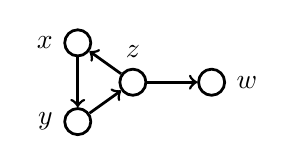
\begin{tikzpicture}[line width = 1pt,
                      solid/.style = {circle, draw, fill = black, minimum size = 0.1cm},
                      empty/.style = {circle, draw, fill = white, minimum size = 0.1cm}]
    \node [empty, label=left:$x$] (a) at (0, 0){};
    \node [empty, label=left:$y$] (b) at (0, -1){};
    \node [empty, label=above:$z$] (c) at (0.7, -0.5){};
    \node [empty, label=right:$w$] (d) at (1.7, -0.5){};
    \draw [->] (c) -- (a);
    \draw [->] (a) -- (b);
    \draw [->] (b) -- (c);
    \draw [->] (c) -- (d);
    \end{tikzpicture} \par
  \end{centering}
  In this graph, there exists a path from $y$ to $w$. If we perform depth-first search on this graph from $z$ in the order $z, x, y, w$, $w$ is visited after the adjacency list of $y$ has been examined, i.e. $\attrib{w}{d} > \attrib{y}{f}$. \par
  \section{[TC] Problem 22.3-12}
  \begin{codebox}
  \Procname{$\proc{DFS}(G)$}
  \zi $\cdots \cdots$
  \setlinenumberplus{}{5}
  \li $c \gets 0$
  \li \For each vertex $u \in \attrib{G}{V}$
  \li \Do  \If $\attrib{u}{color} \isequal \const{white}$
  \li      \Do $c \gets c + 1$
  \li          $\proc{DFS-Visit}(G, u, c)$
           \End
      \End
  \end{codebox}
  \begin{codebox}
  \Procname{$\proc{DFS-Visit}(G, u, c)$}
  \zi $\cdots \cdots$
  \setlinenumberplus{}{4}
  \li $\attrib{u}{cc} \gets c$
  \li \For each vertex $v \in \attrib{G}{Adj}[u]$
  \li \Do  \If $\attrib{u}{color} \isequal \const{white}$
  \li      \Do $\attrib{v}{\pi} \gets u$
  \li          $\proc{DFS-Visit}(G, v, c)$
           \End
      \End
  \zi $\cdots \cdots$
  \end{codebox}

  \section{[TC] Problem 22.4-2}
  \begin{codebox}
  \Procname{$\proc{Count-Simple-Paths}(G, s, t)$}
  \li \For each vertex $u \in \attrib{G}{V}$
  \li \Do  $\id{count}[u] \gets 0$
      \End
  \li $\id{count}[s] \gets 1$
  \li $T \gets \proc{Topological-Sort}(G)$
  \li $x \gets \attrib{T}{head}$
  \li \While $x \neq \NIL$
  \li \Do \For each vertex $v \in \attrib{G}{Adj}[\attrib{x}{key}]$
  \li     \Do $\id{count}[v] \gets \id{count}[v] + \id{count}[\attrib{x}{key}]$
          \End
  \li     $x \gets \attrib{x}{next}$
      \End
  \li \Return $\id{count}[t]$
  \end{codebox}

  \section{[TC] Problem 22.4-3}
  We can modify DFS to determine whether the undirected graph contains a cycle.
  \begin{codebox}
  \Procname{$\proc{DFS}(G)$}
  \zi $\cdots \cdots$
  \setlinenumberplus{}{5}
  \li \For each vertex $u \in \attrib{G}{V}$
  \li \Do  \If $\attrib{u}{color} \isequal \const{white}$
  \li          $\proc{DFS-Visit}(G, u, \NIL)$
           \End
      \End
  \li print ``does not contain a cycle''
  \end{codebox}
  \begin{codebox}
  \Procname{$\proc{DFS-Visit}(G, u, p)$}
  \zi $\cdots \cdots$
  \setlinenumberplus{}{4}
  \li $\attrib{u}{cc} \gets c$
  \li \For each vertex $v \in \attrib{G}{Adj}[u]$
  \li \Do  \If $\attrib{u}{color} \isequal \const{white}$
  \li      \Do $\attrib{v}{\pi} \gets u$
  \li          $\proc{DFS-Visit}(G, v, u)$
  \li      \ElseIf $v \neq p$
  \li      \Do print ``contains a cycle''
  \li          terminate DFS
           \End
      \End
  \zi $\cdots \cdots$
  \end{codebox}
  In this algorithm, every vertex is visited at most once. If a vertex is to be visited for the second time, it means that the graph contains a cycle, and the procedure will be immediately terminated. Hence the algorithm run in $O(|V|)$ time, independent of $|E|$.

  \section{[TC] Problem 22.5-5}
  \begin{codebox}
  \Procname{$\proc{Component-Graph}(G)$}
  \li compute the strongly connected components of $G$
  \li assign each vertex $v$ an integer label $\attrib{v}{scc}$ between 1 and $k$, denoting which strongly \\ connected components $v$ belongs to, where $k$ is the number of the components.
  \li $\attrib{G^{\id{scc}}}{V} \gets\{1, 2, \cdots, k\}$
  \li \For each edge $(u, v) \in \attrib{G}{E}$
  \li \Do \If $\attrib{u}{scc} \neq \attrib{v}{scc}$
  \li     \Do $\attribb{G^{\id{scc}}}{E}{insert}((\attrib{u}{scc}, \attrib{v}{scc}))$
          \End
      \End
  \zi \Comment use radix sort to sort the edges
  \li perform counting sort on $\attrib{G^{\id{scc}}}{E}$, using the second endpoint of each edge as key
  \li perform counting sort on $\attrib{G^{\id{scc}}}{E}$, using the first endpoint of each edge as key
  \li delete the consecutive duplicate edges in ($\attrib{G^{\id{scc}}}{E}$) \Comment after sorting, duplicate edges must be consecutive
  \zi \Comment construct adjacency lists
  \li \For each edge $(u, v) \in \attrib{G^{\id{scc}}}{E}$
  \li \Do  $\attribb{G^{\id{scc}}}{Adj[u]}{insert}(v)$
      \End
  \li \Return $G^{\id{scc}}$
  \end{codebox}
  In this procedure, line 1, line 2, line 3-6, line 7, line 8, line 9, line 10-11 cost $O(|V|+|E|)$ time respectively, and thus the algorithm takes a total running time of $O(|V|+|E|)$.

  \section{[TC] Problem 22.5-6}
  \begin{codebox}
  \Procname{$\proc{Is-Semiconnected}(G)$}
  \li $G^{\id{scc}} \gets \proc{Component-Graph}(G)$
  \li $T \gets \proc{Topological-Sort}(G^{\id{scc}})$
  \li \For $i \gets 1$ \To $\attrib{T}{length} - 1$
  \li \Do  \If $(T[i], T[i+1]) \notin \attrib{G^{\id{scc}}}{E}$
  \li      \Do \Return \const{false}
           \End
      \End
  \li \Return \const{true}
  \end{codebox} \par
  In this procedure, line 1, line 2 takes a running time of $O(|V|+|E|)$, respectively. Line 3-4 takes a running time of $O(1 + \od(v))$ for each vertex $v$ to verify whether or not $(T[i], T[i+1]) \in \attrib{G^{\id{scc}}}{E}$, where $\od(v)$ is the out-degree of $v$, and $O(|V|+|E|)$ in sum. Therefore, the total running time is $O(|V|+|E|)$. \par
  We break the proof of the correctness of this algorithm into the two steps: \par
  \textbf{Step 1:} A graph $G$ is semiconnected if and only if its component graph $G^{\id{scc}}$ is semiconnected. \par
  \emph{Proof} `if': for every two distinct nodes $u, v$ in $G$, if they are in the same strongly connected component, then they are semiconnected; otherwise, let $u \in C_1$, $v \in C_2$, where $C_1, C_2$ are two distinct strongly connected components. Since the component graph is semiconnected, we have $C_1 \rightsquigarrow C_2$ or $C_2 \rightsquigarrow C_1$. Without loss of generality, assume $C_1 \rightsquigarrow C_2$. For every edge $(C_i, C_j)$ in the path $C_1 \rightsquigarrow C_2$, replace it with two vertices $u \in C_i, v \in C_j$, where $(u, v) \in G$. For every two incident edges $(C_i, C_j), (C_j, C_k)$ and their corresponding vertices $u \in C_i, v, w \in C_j, x \in C_k$, since $v$ and $w$ are in the same component, we can add a path $v \rightsquigarrow w$ between $v$ and $w$. Finally, we get a path from $u$ to $v$. Therefore, $G$ is semiconnected.  \par
  `only if': for every two distinct nodes $C_1, C_2$ in $G^{\id{scc}}$, choose two elements $x \in C_1, y \in C_2$, then $x \rightsquigarrow y$ or $y \rightsquigarrow x$. Replace each node in $x \rightsquigarrow y$ (or $y \rightsquigarrow x$) with the component it belongs to, we obtain a path, or more precisely, a walk from $C_1$ to $C_2$ (or from $C_2$ to $C_1$), therefore $G^{\id{scc}}$ is semiconnected. \par
  \textbf{Step 2:} A DAG $G$ is semiconnected if and only if for every two vertices $u, v$ adjacent in the topological sort $G$, then $u$ and $v$ are connected by a directed edge in $G$. \par
  \emph{Proof} `if': for every distinct vertices $u, v$, assume, without loss of generality, that $u$ appears before $v$ in the topological sort, i.e. the topological sort is $\cdots, u, w_1, w_2, \cdots, w_n, v, \cdots$, then $(u, w_1), (w_1, w_2), \cdots, (w_n, v)$ are directed edges in $G$, i.e. $u \rightsquigarrow v$. Therefore, $G$ is semiconnected. \par
  `only if': suppose, to the contrary, that there exists two vertices $u, v$ adjacent in the topological sort $G$, but $u$ and $v$ are not connected by a directed edge in $G$. It is impossible that $v \rightsquigarrow u$, because $u$ appears before $v$. Therefore $u \rightsquigarrow v$. Since they are not connected by a directed edge, the path from $u$ to $v$ must contain at least 3 vertices, i.e. there must exist another vertex $w$, such that $u \rightsquigarrow w \rightsquigarrow v$. By the property of topological sort, $w$ appears after $u$ but before $v$. However, $u$ and $v$ are adjacent in the topological sort, which leads to contradiction. \par
  Note that the component graph is a DAG. Combine the two steps, we obtain a complete proof of the correctness of the algorithm.
\end{document}
